  
  \begin{figure}[!htbp]
  \centering
  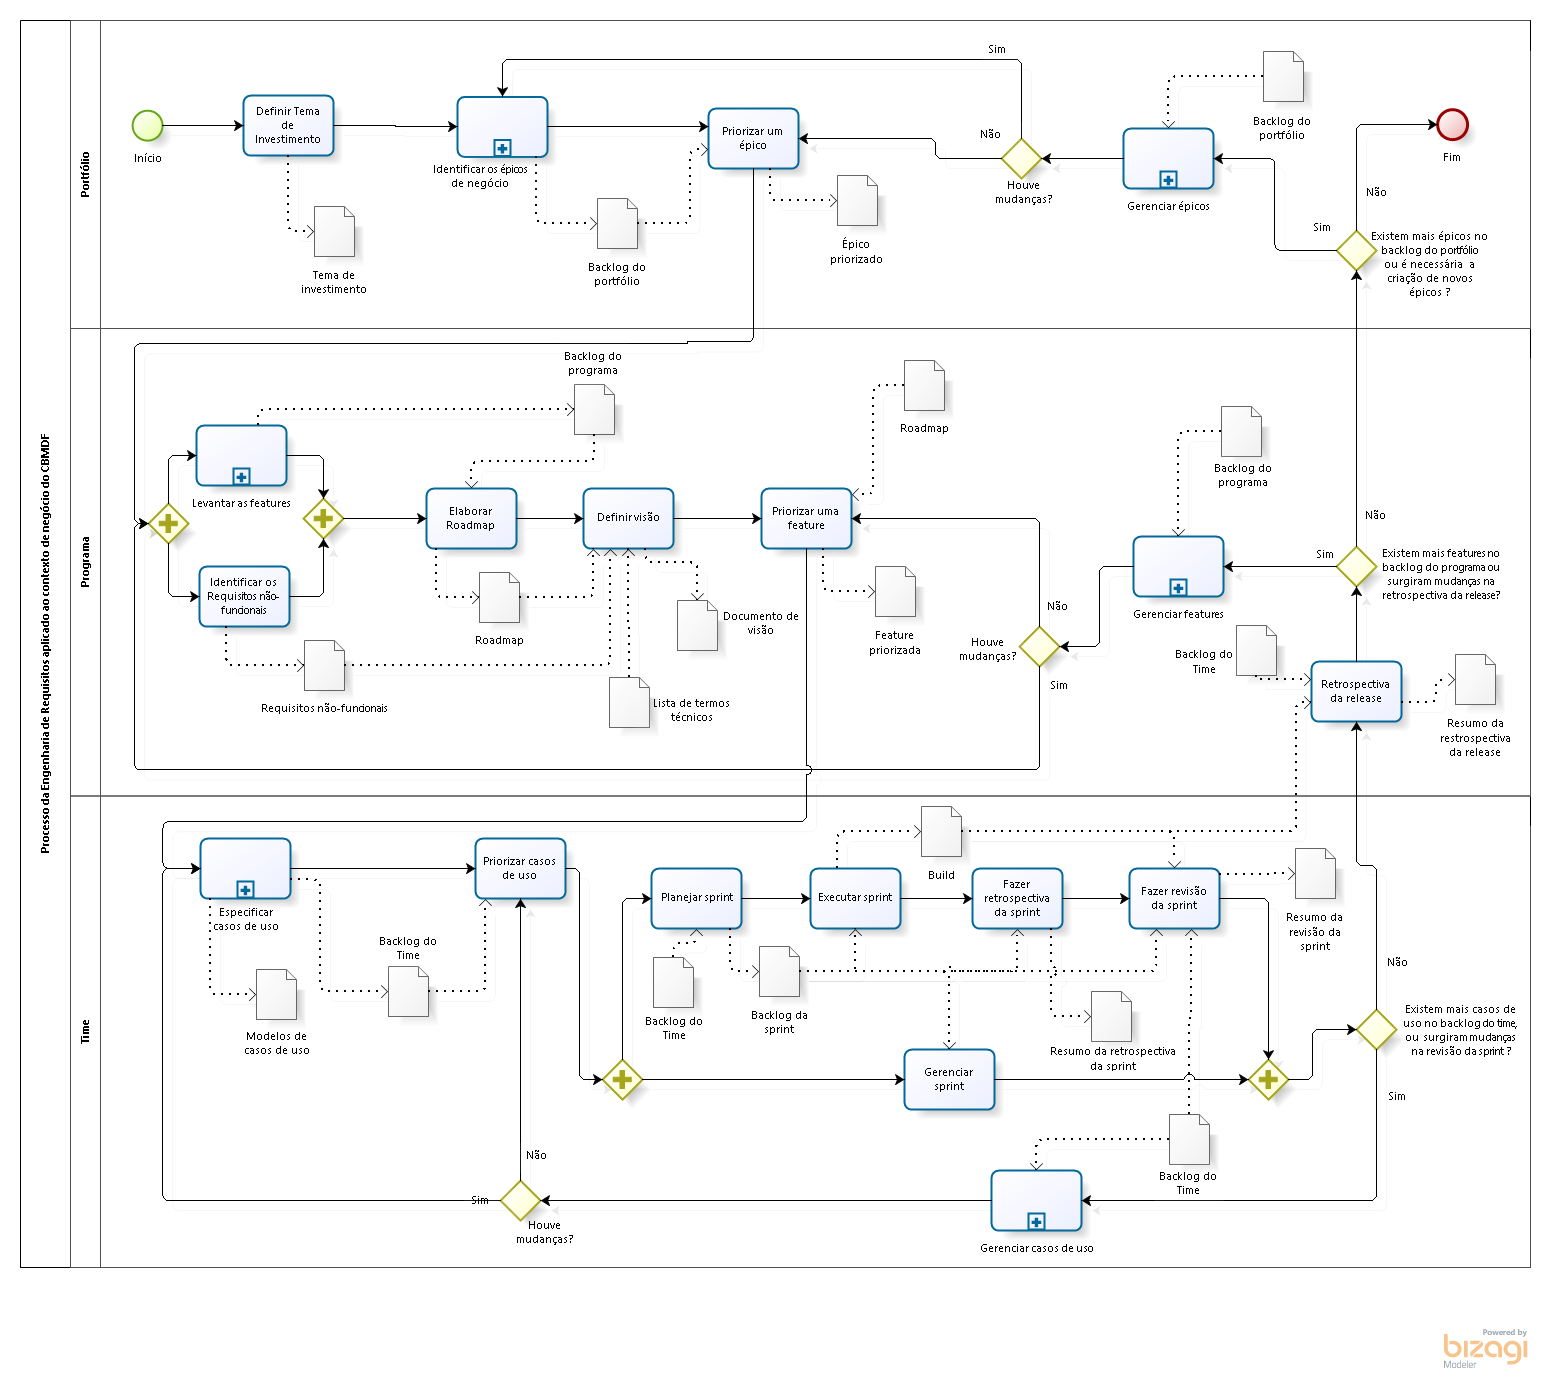
\includegraphics[scale=0.5, angle = 90]{editaveis/figuras/project_big_picture}
  \caption[Modelo do processo de Engenharia de Requisitos: \textit{Big Picture} do projeto]
      {Modelo do processo de Engenharia de Requisitos: \textit{Big Picture} do projeto.}
  \label{project_big_picture}
  \end{figure}
  
  \pagebreak
  \subsection{Subprocessos da '\textit{Big Picture}' do projeto}

    \begin{figure}[!htbp]
      \centering
      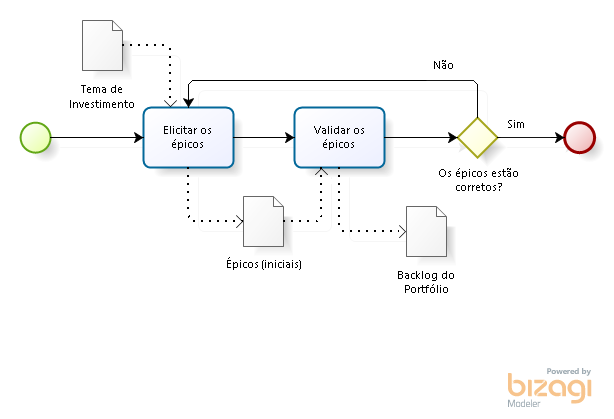
\includegraphics[scale=0.55]{editaveis/figuras/processo_identificar_epicos}
      \caption[Subprocesso - Identificar épicos de negócio]{Subprocesso - Identificar épicos de negócio.}
      \label{processo_identificar_epicos}
    \end{figure}

    \begin{figure}[!htbp]
      \centering
      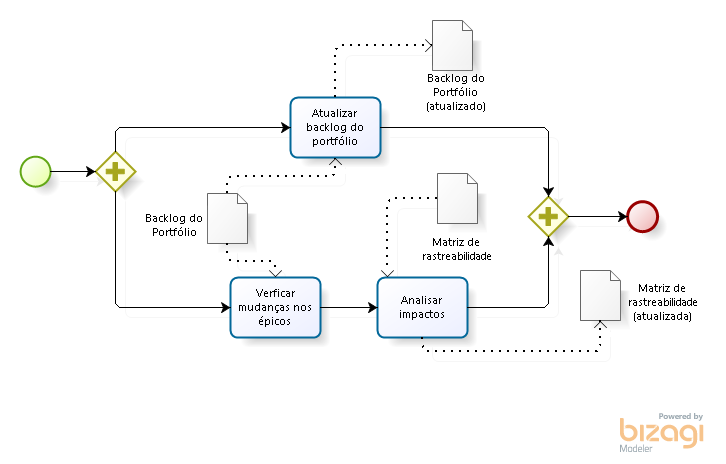
\includegraphics[scale=0.55]{editaveis/figuras/processo_gerenciar_epicos}
      \caption[Subprocesso - Gerenciar épicos]{Subprocesso - Gerenciar épicos.}
      \label{processo_gerenciar_epicos}
    \end{figure}

    \begin{figure}[!htbp]
      \centering
      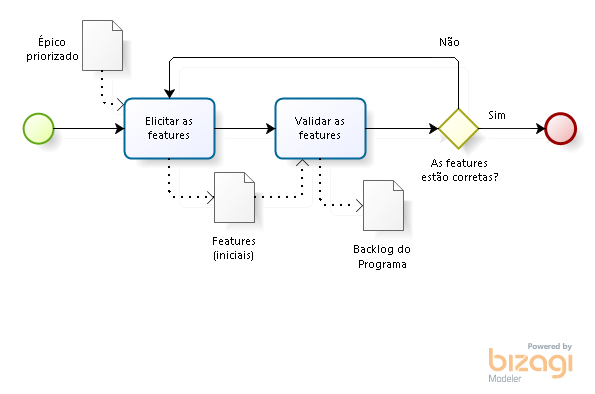
\includegraphics[scale=0.55]{editaveis/figuras/processo_levantar_features}
      \caption[Subprocesso - Levantar \textit{features}]{Subprocesso - Levantar \textit{features}.}
      \label{processo_levantar_features}
    \end{figure}

    \pagebreak
    \begin{figure}[!htbp]
      \centering
      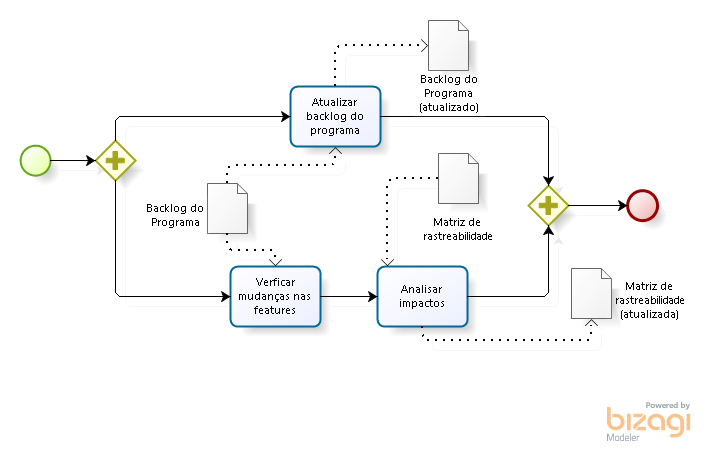
\includegraphics[scale=0.55]{editaveis/figuras/processo_gerenciar_features}
      \caption[Subprocesso - Gerenciar \textit{features}]{Subprocesso - Gerenciar \textit{features}.}
      \label{processo_gerenciar_features}
    \end{figure}

    \begin{figure}[!htbp]
      \centering
      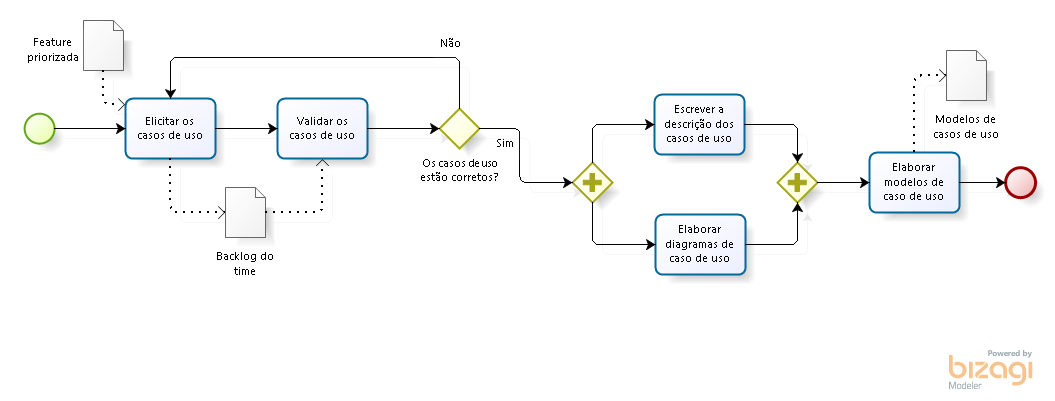
\includegraphics[scale=0.55]{editaveis/figuras/processo_especificar_casos_uso}
      \caption[Subprocesso - Especificar casos de uso]{Subprocesso - Especificar casos de uso.}
      \label{processo_especificar_casos_uso}
    \end{figure}

    \begin{figure}[!htbp]
      \centering
      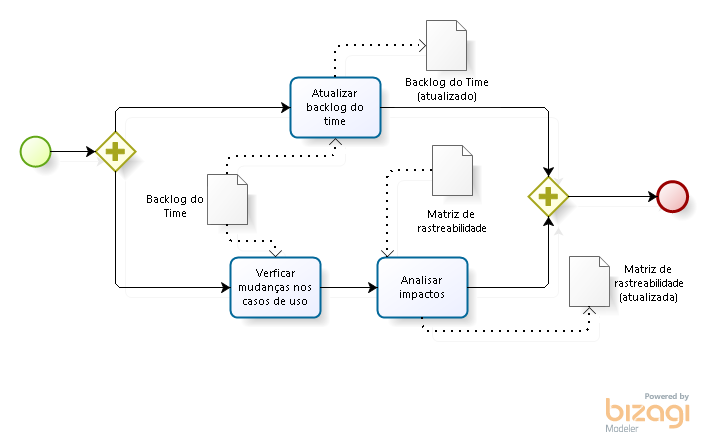
\includegraphics[scale=0.55]{editaveis/figuras/processo_gerenciar_casos_uso}
      \caption[Subprocesso - Gerenciar casos de uso]{Subprocesso - Gerenciar casos de uso.}
      \label{processo_gerenciar_casos_uso}
    \end{figure}